\documentclass[12pt,norsk,a4paper]{article}
\usepackage[norsk]{babel}
\usepackage[norsk]{isodate}
\usepackage[T1]{fontenc}
\usepackage{parskip}
\usepackage{url}
\usepackage{cancel}
\usepackage{mathtools}
\usepackage{xfrac}
\usepackage{listings}
\author{Frida Berge (fridatbe)}
\title{IN3140 --- Obligatorisk oppgåve 4}
\date{\today}
\usepackage[small,euler-digits]{eulervm}
\usepackage{color}
% \usepackage{minted}
\usepackage{xcolor}
\definecolor{LightGray}{gray}{0.9}
\usepackage{a4wide}
\usepackage[top=2cm]{geometry}
\usepackage{graphicx}
\graphicspath{ {./fig/} }
\newcommand{\tuple}[1]{\ensuremath{\langle #1\rangle}}
\newcommand{\set}[1]{\ensuremath{\{#1\}}}
\newcommand{\imp}{\ensuremath{\rightarrow}}
\newcommand{\M}{\ensuremath{\mathcal{M}}}
\newcommand{\AF}{edge from parent[draw=none]}
\newcommand{\NODE}[1]{\{node \{\ensuremath{#1}\}\}}
\usepackage[explicit]{titlesec}
\titleformat{\section}{\normalfont\Large\bfseries}{}{0em}{#1\ \thesection}
\begin{document}
    \maketitle
    \renewcommand{\thesubsection}{(\alph{subsection})}



    \newpage
    \section{Oppgåve}
    \textbf{1a)}\\
    Gjer om til 1DOF og reknar ut poteniell og kinetisk energi:\\
    Reknar ut potensiell energi ($\theta$ er lik $\theta_2$ frå gamal notasjon, og m er lik $m_2+m_3$):
    \[P = mgh = mgL\cos(\theta)\]

    Reknar ut kinetisk energi (L er lik $L_2+L_3$ frå gamal notasjon, og $R_1^0$ er lik $R_2^0$ frå gamal notasjon i oblig 3):
    \[\frac{m\dot\theta^2L^2}{2}+\frac{\left[\begin{array}{ccc}0 & 0 & \dot\theta\end{array}\right](R_1^0)(I_2+I_3)(R_1^0)^T\left[\begin{array}{c}0 \\ 0 \\ \dot\theta\end{array}\right]}{2}\]
    \[=\frac{m\dot\theta^2L^2}{2}+\frac{\left[\begin{array}{ccc}0 & 0 & \dot\theta\end{array}\right]\left[\begin{array}{ccc}c(\theta) & -s(\theta) & 0 \\ s(\theta) & c(\theta) & 0 \\ 0 & 0 & 1\end{array}\right](I_2+I_3)\left[\begin{array}{ccc}c(\theta) & -s(\theta) & 0 \\ s(\theta) & c(\theta) & 0 \\ 0 & 0 & 1\end{array}\right]^T\left[\begin{array}{c}0 \\ 0 \\ \dot\theta\end{array}\right]}{2}\]
    \[=\frac{m\dot\theta^2L^2}{2}+ \frac{I_{2,zz}+I_{3,zz}\dot\theta^2}{2}\]

    Dette gir:
    \[\mathcal{L} = K-P = \frac{m\dot\theta^2L^2}{2}+ \frac{(I_{2,zz}+I_{3,zz})\dot\theta^2}{2} - mgL\cos(\theta)\]

    Dette gir utrykk for $\tau$:
    \[\tau = \frac{d}{dt}\frac{\partial\mathcal{L}}{\partial\dot\theta}-\frac{\partial\mathcal{L}}{\partial\theta}\]
    \[\frac{\partial\mathcal{L}}{d\dot\theta} = mL^2\dot\theta + (I_{2,zz}+I_{3,zz})\dot\theta\]
    \[\frac{d}{dt}\frac{\partial\mathcal{L}}{\partial\dot\theta} = mL^2\ddot\theta + (I_{2,zz}+I_{3,zz})\ddot\theta\]
    \[\frac{\partial\mathcal{L}}{\partial\theta} = mgL\sin(\theta)\]
    \[\tau = mL^2\ddot\theta + (I_{2,zz}+I_{3,zz})\ddot\theta - mgL\sin(\theta)\]
    \[\tau = \ddot\theta(mL^2 + (I_{2,zz}+I_{3,zz})) - mgL\sin(\theta)\]

    Skriv om $(I_{2,zz}+I_{3,zz})$ til $I_{zz}$:
    \[\tau = \underline{\ddot\theta(mL^2 + I_{zz}) - mgL\sin(\theta)}\]

    \textbf{1b)}\\
    \[u(t) = J\ddot\theta(t)+B\dot\theta(t)+D(t)\]
    \[U(s) = Js^2\theta+Bs\theta+D\]
    Der J, B og D representerar:
    \[J = mL^2 + I_{zz} \hspace{10mm} B = 0 \hspace{10mm} D = -mgL\sin(\theta)\]

    \textbf{1c)}\\
    \[U(s) = Js^2\theta + Bs\theta + D\]
    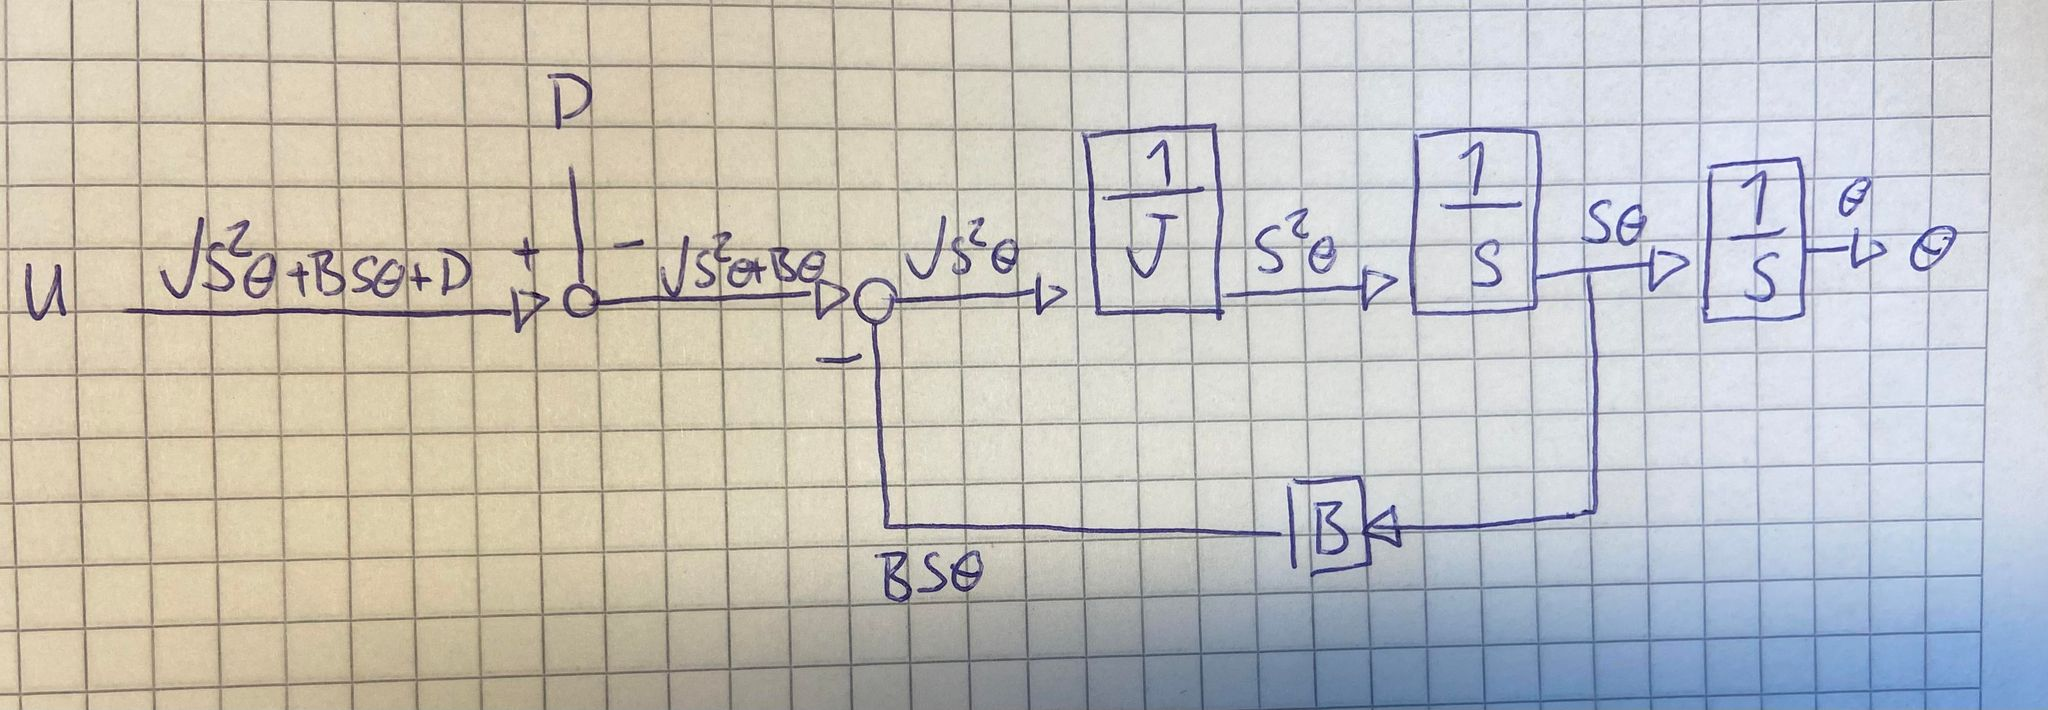
\includegraphics[width=0.8\textwidth]{tegning.jpg}\\
    PD-kontroller:
    \[U(s) = (K_p+sK_d)E(t)\]
    \[U(s) = (K_p+sK_d)(\theta_d - \theta)\]
    \[U(s) = K_p\theta_d - K_p\theta + sK_d\theta_d - sK_d\theta\]
    Ved start er $s\theta_d = 0$:
    \[U(s) = K_p\theta_d - K_p\theta - sK_d\theta\]

    Finner eit utrykk for $\theta$ aleine:\\
    \[Js^2\theta + Bs\theta + D = K_p\theta_d - K_p\theta - sK_d\theta\]
    \[Js^2\theta + Bs\theta + K_p\theta + sK_d\theta = K_p\theta_d - D \]
    \[\theta(Js^2 + Bs + K_p + sK_d) = K_p\theta_d - D \]
    \[\theta = \frac{K_p\theta_d - D}{Js^2 + Bs + K_p + sK_d} \]
    

    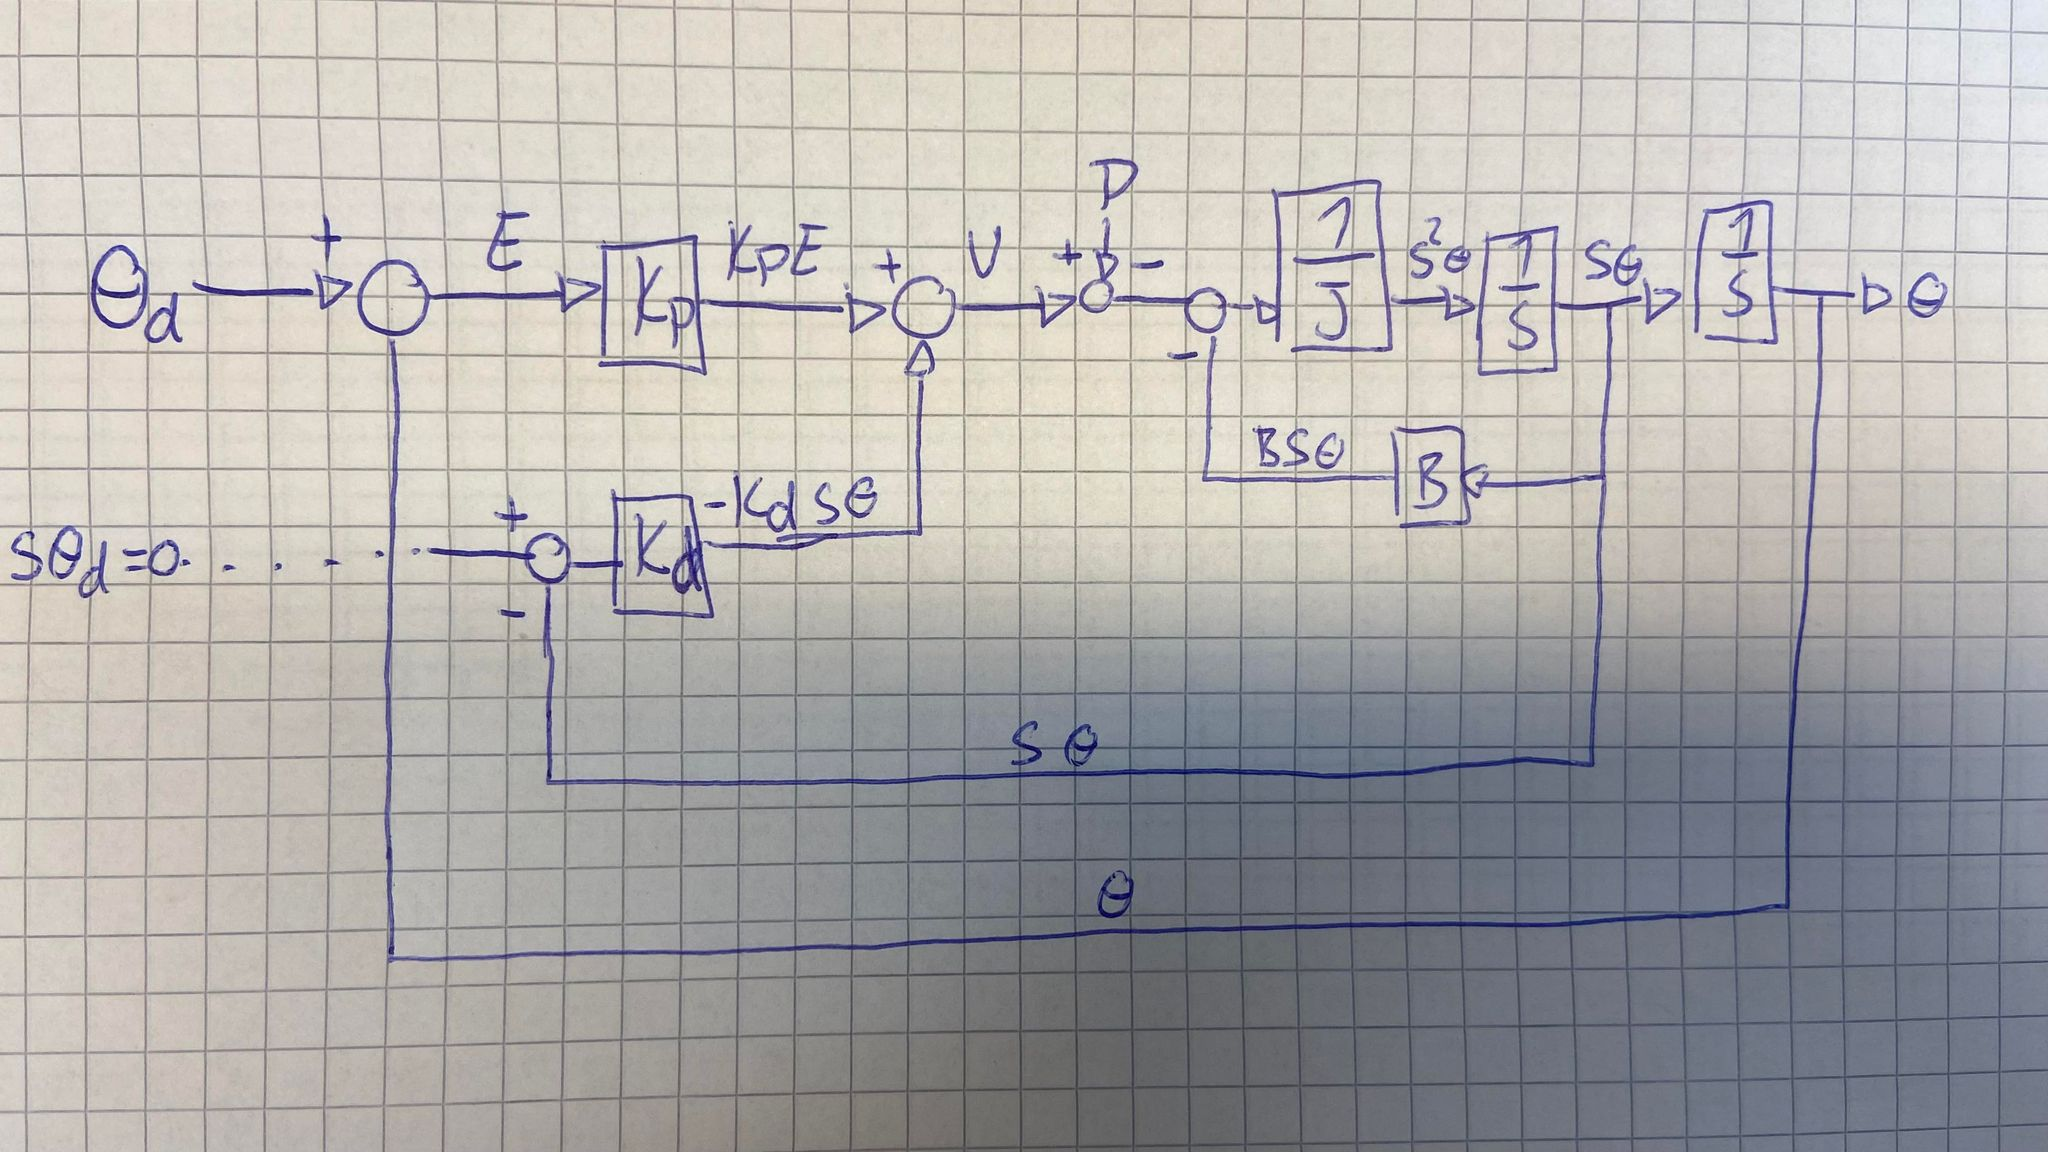
\includegraphics[width=0.8\textwidth]{tegning2.jpg}\\

    \textbf{1c)}\\
    Ved kritisk dempa system er $zeta = 1$ og $\omega$ er oppgitt i oppgåva:
    \[\zeta = 1 \hspace{10mm} \omega = 6\]
    Frå boka har vi at $K_p$ og $K_d$ finnes frå utrykket:
    \[s^2+\frac{B+K_d}{J}s+\frac{K_p}{J} = s^2+s\zeta\omega+\omega^2\]
    \[K_p = \omega^2J \hspace{10mm} K_d = 2\zeta\omega J-B\]
    Fyller vi inn verdiane for $\zeta$ og $\omega$ får vi:
    \[K_p = 6^2J = 36J = 36(mL^2+I_{zz})\]
    \[K_p = 36(0.413*0.128+5.126) = \underline{186.43}\]
    \[K_d = 12J-B = 12(mL^2+I_{zz})-0 = 12(mL^2+I_{zz})\]
    \[K_d = 12J-B = 12(mL^2+I_{zz})-0 = 12(0.413*0.128+5.126) = \underline{62.14}\]

    \newpage
    \section{Oppgåve}
    \textbf{2a)}\\
    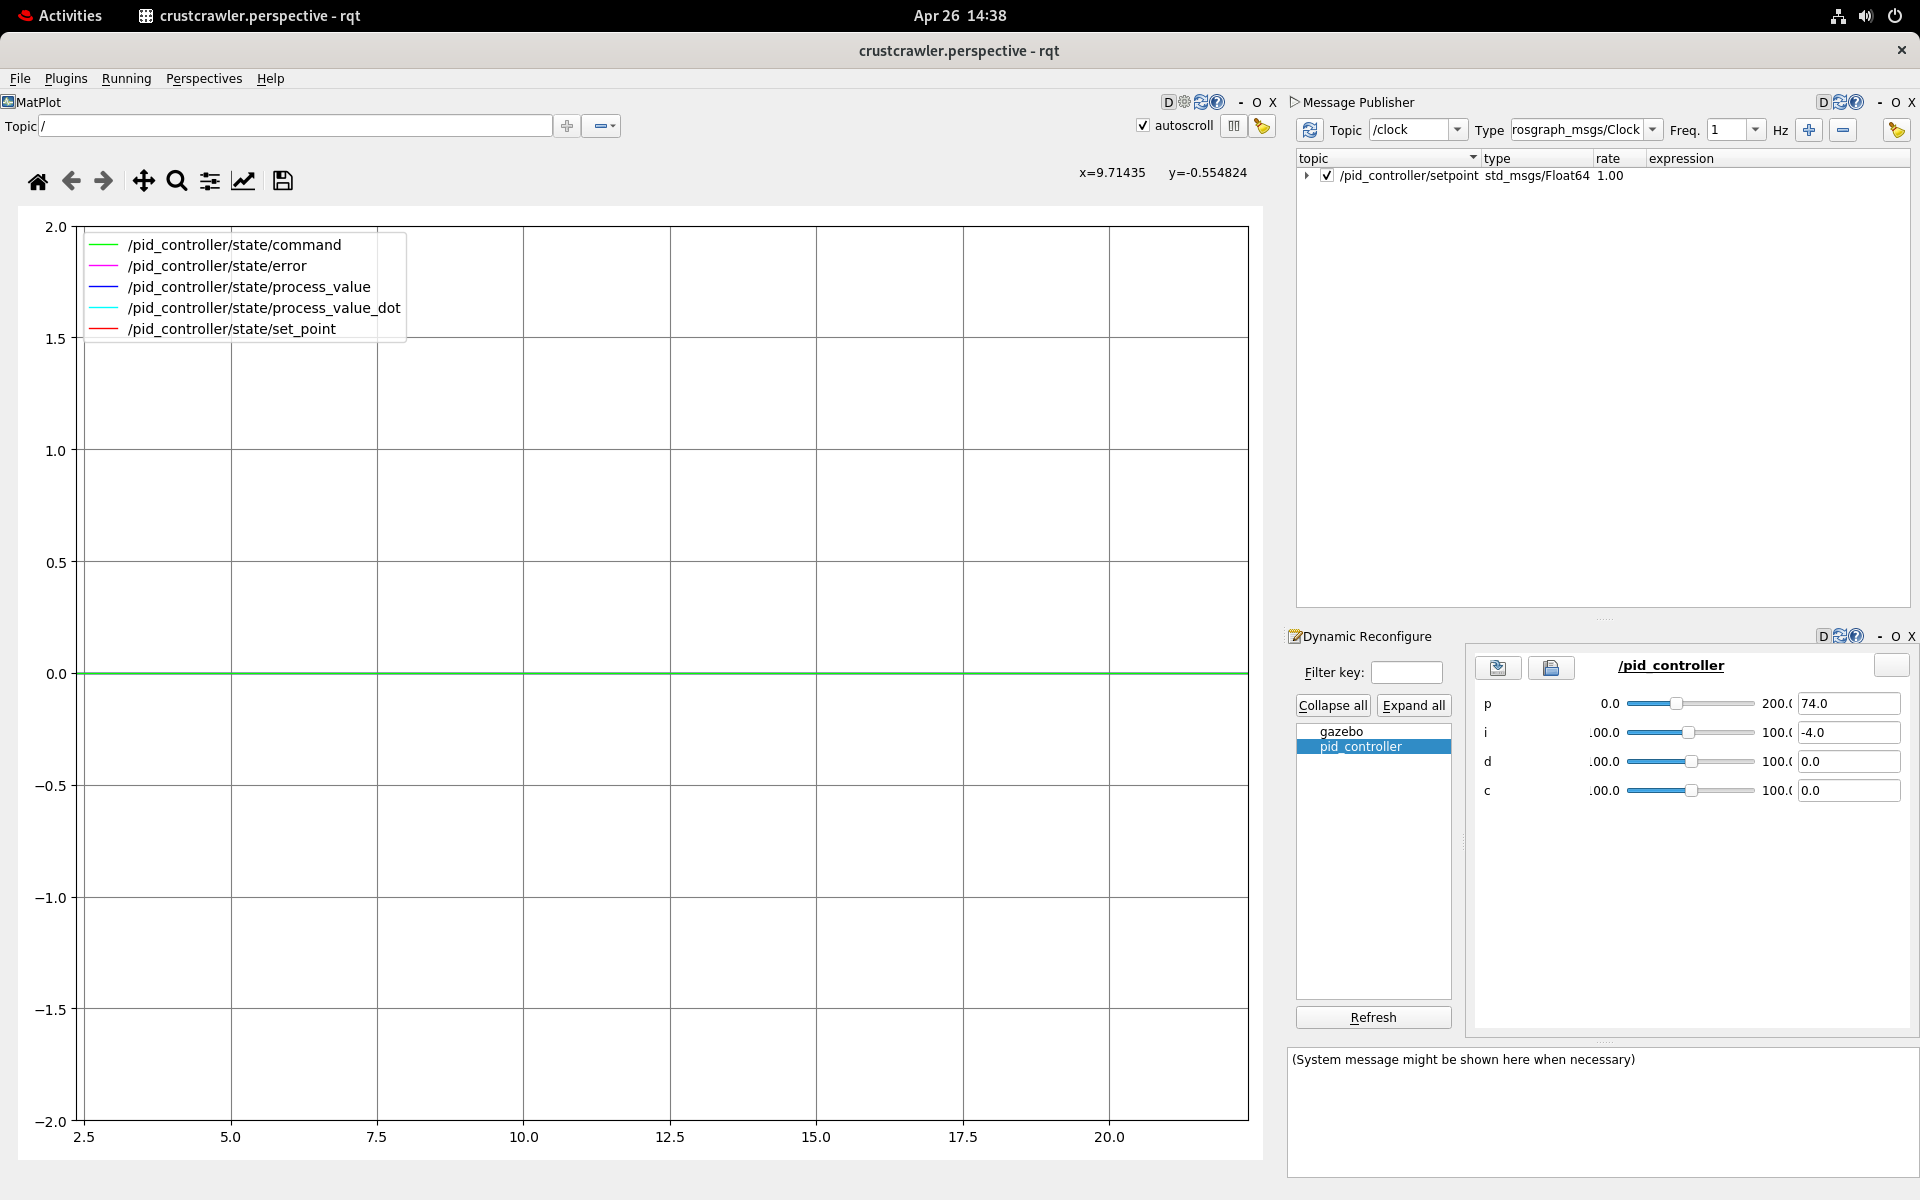
\includegraphics[width=0.8\textwidth]{bilde1.png}\\
    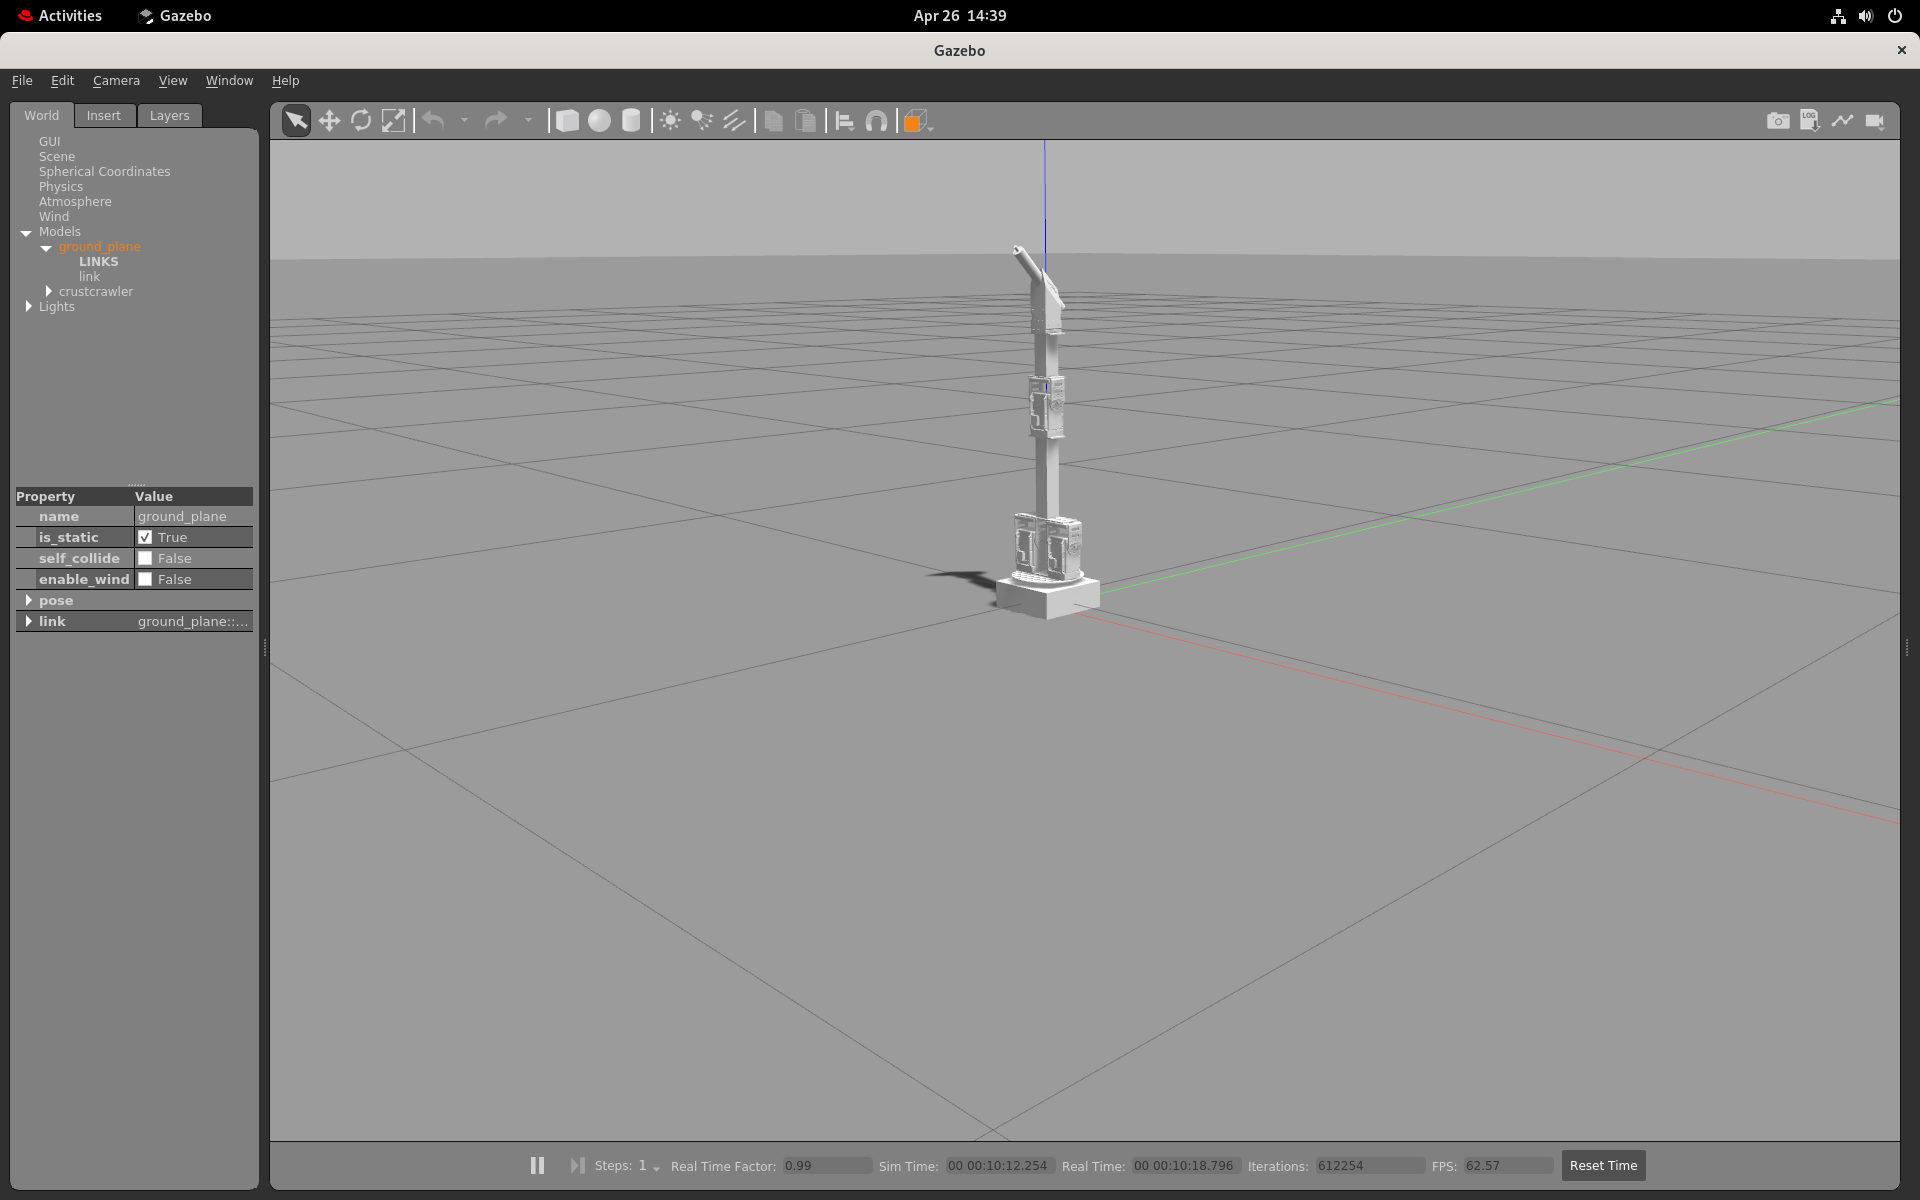
\includegraphics[width=0.8\textwidth]{bilde2.png}\\



    \newpage
    \section{Oppgåve}
    \textbf{3a)}\\
    Forventa 'settling time':
    \[t_s = \frac{4}{\zeta\omega} = \frac{4}{1*6} = 0.667s\]
    Verkeleg 'settling time' ($5\%$ før 1.024 er er 1.0235):
    \[t_s = 28-27.5 = \underline{0.5s}\]
    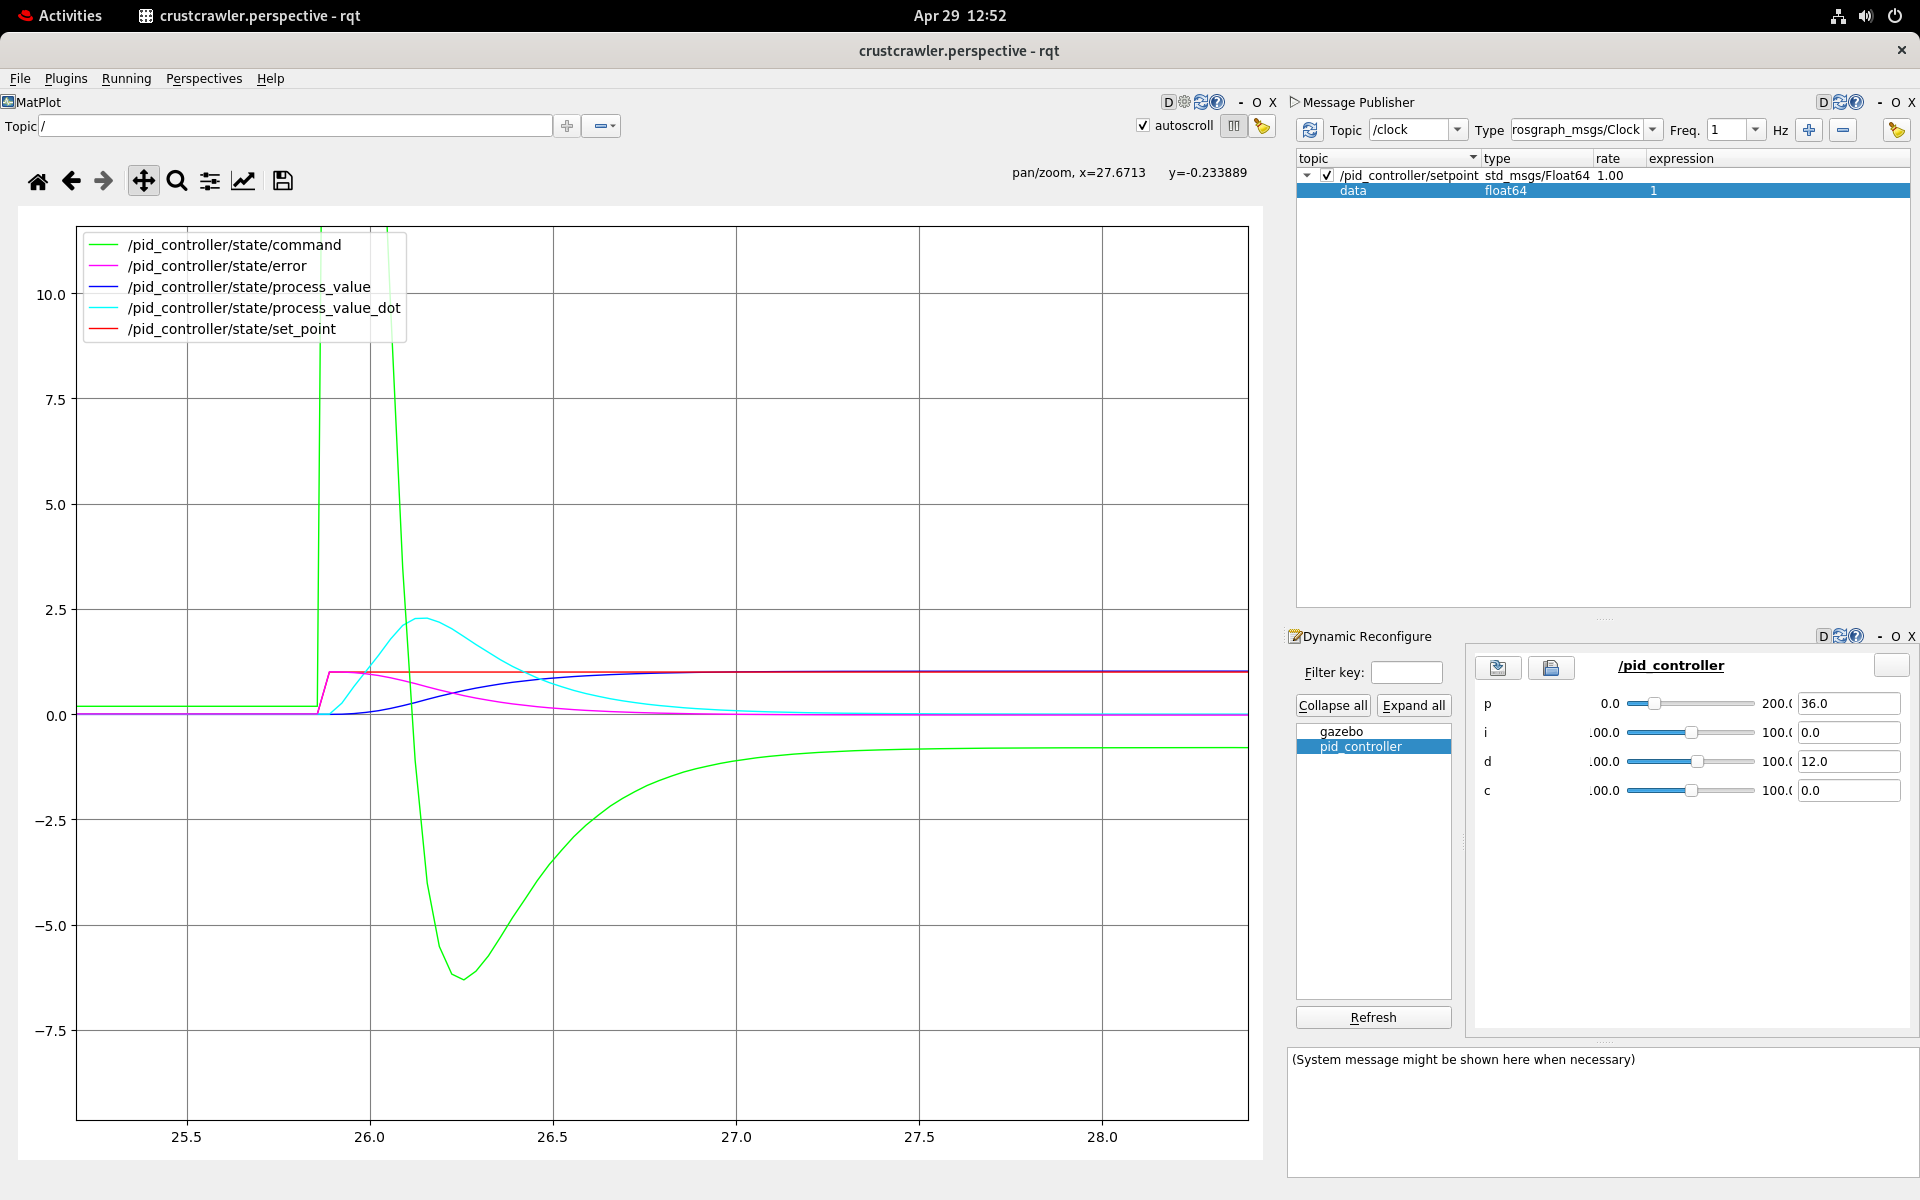
\includegraphics[width=0.8\textwidth]{graf.png}\\
    Eg brukte P = 36 og D = 12 sjølv om eg rekna ut dei faktiske verdiane i oppgåve 1.
    Eg valte likeveol å bruke dei to tala fordi forhaldet mellom dei fortsatt er det same, og da unngår eg avrundingsfeil ved utregning


    \textbf{3b)}\\
    Minste 'settling time' eg fann var 0.16s, da var sett-punkt-mistak på 0.019s.
    Da var verdiane på $K_p$ = 56 og $K_d = 12$\\
    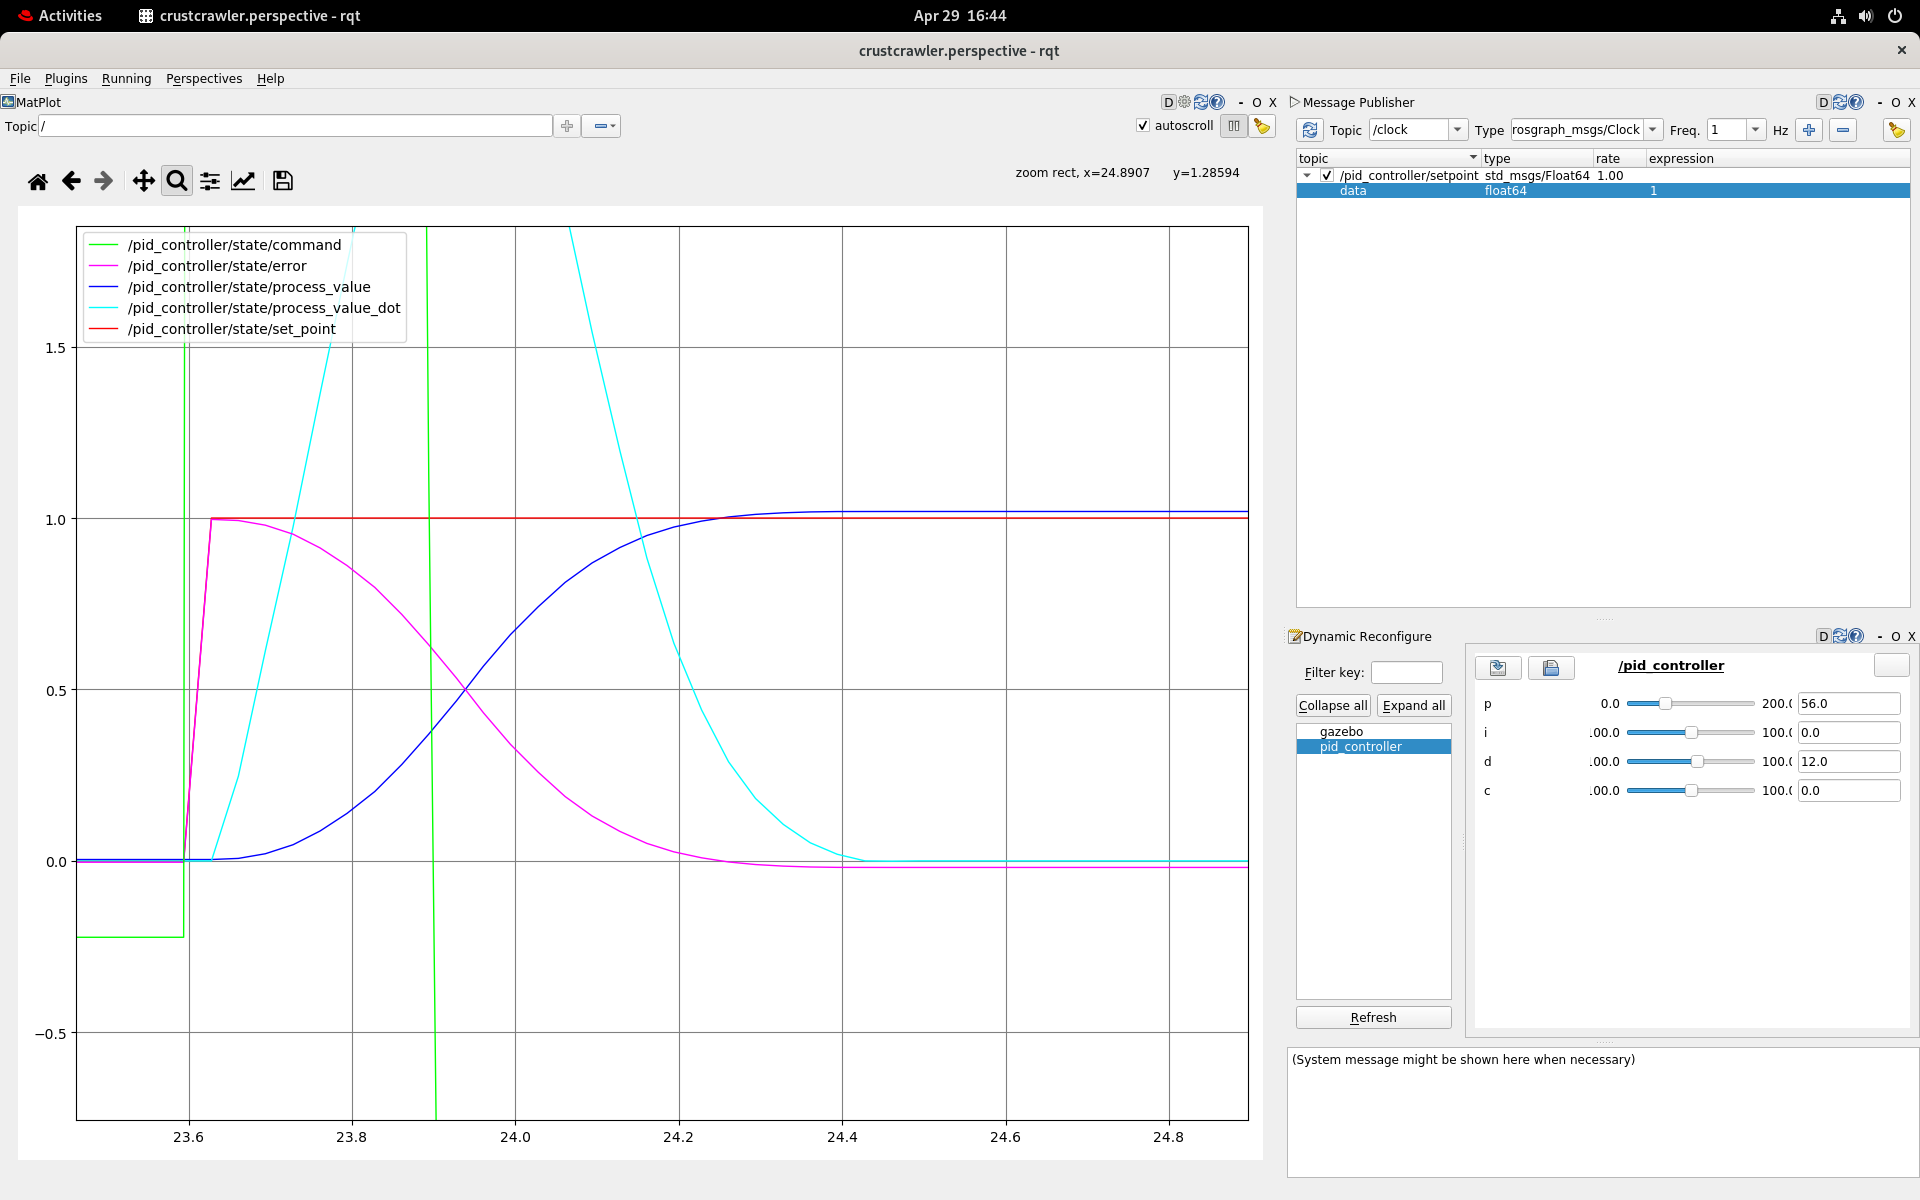
\includegraphics[width=0.8\textwidth]{best_set.png}\\


    \textbf{3c)}\\
    Eg synes feilmargina var svært liten, men dersom eg skulle ha gjort den enda mindre ville eg implementert ei PID kontrollar (eg skrev koden i pid.py) slik at kontrollaren også tek hensyn til akumullert feilmargin over tid

    \textbf{3d)}\\
    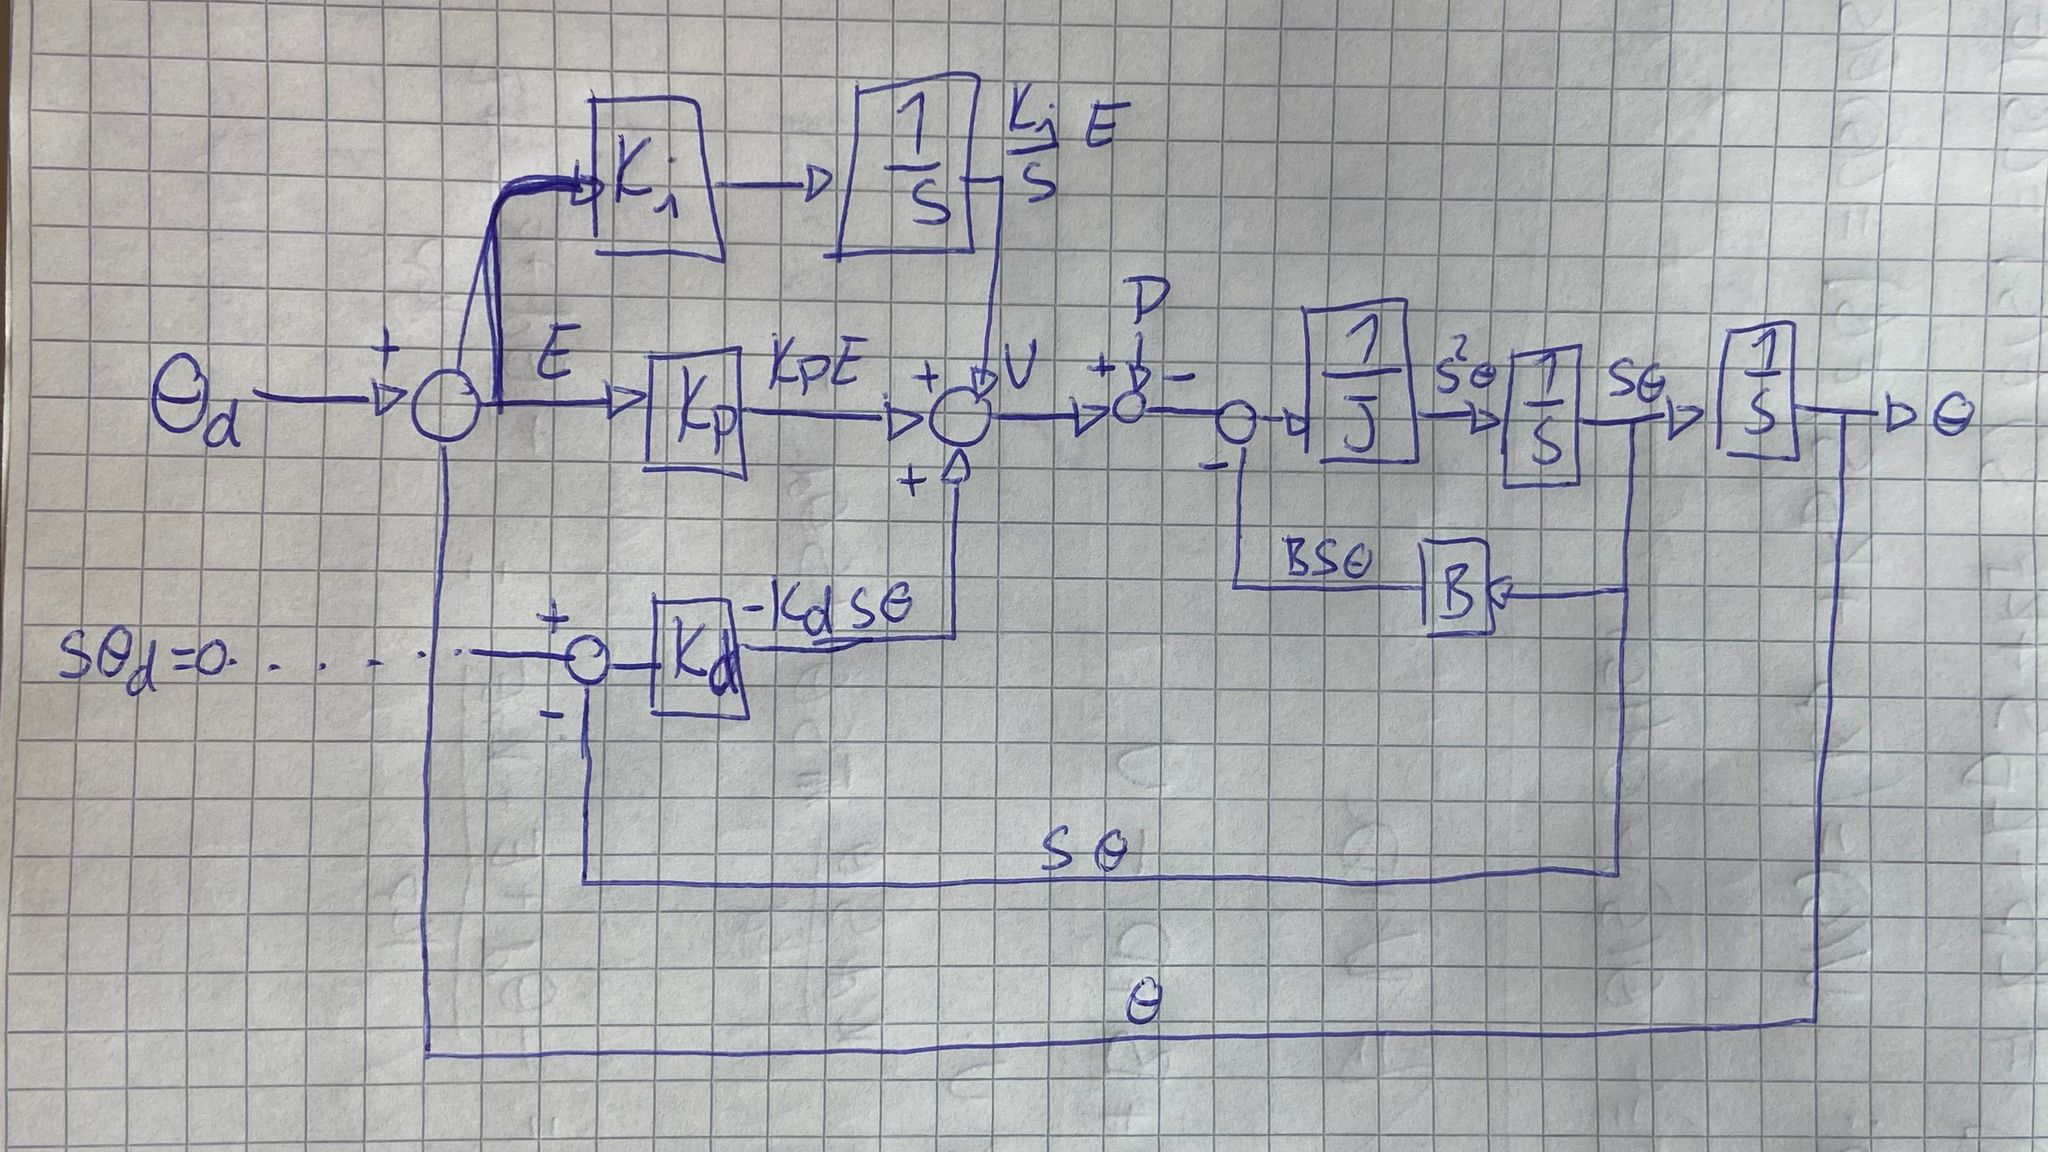
\includegraphics[width=0.8\textwidth]{tegning3.jpg}\\

    \newpage
    \section{Oppgåve}
    \textbf{4a)}\\
    Implementeringa ligg i  kodefila pid.py under $PI\_ctrl$\\
    


    \textbf{4b)}\\
    Beste justeringa eg fann sjølv:\\
    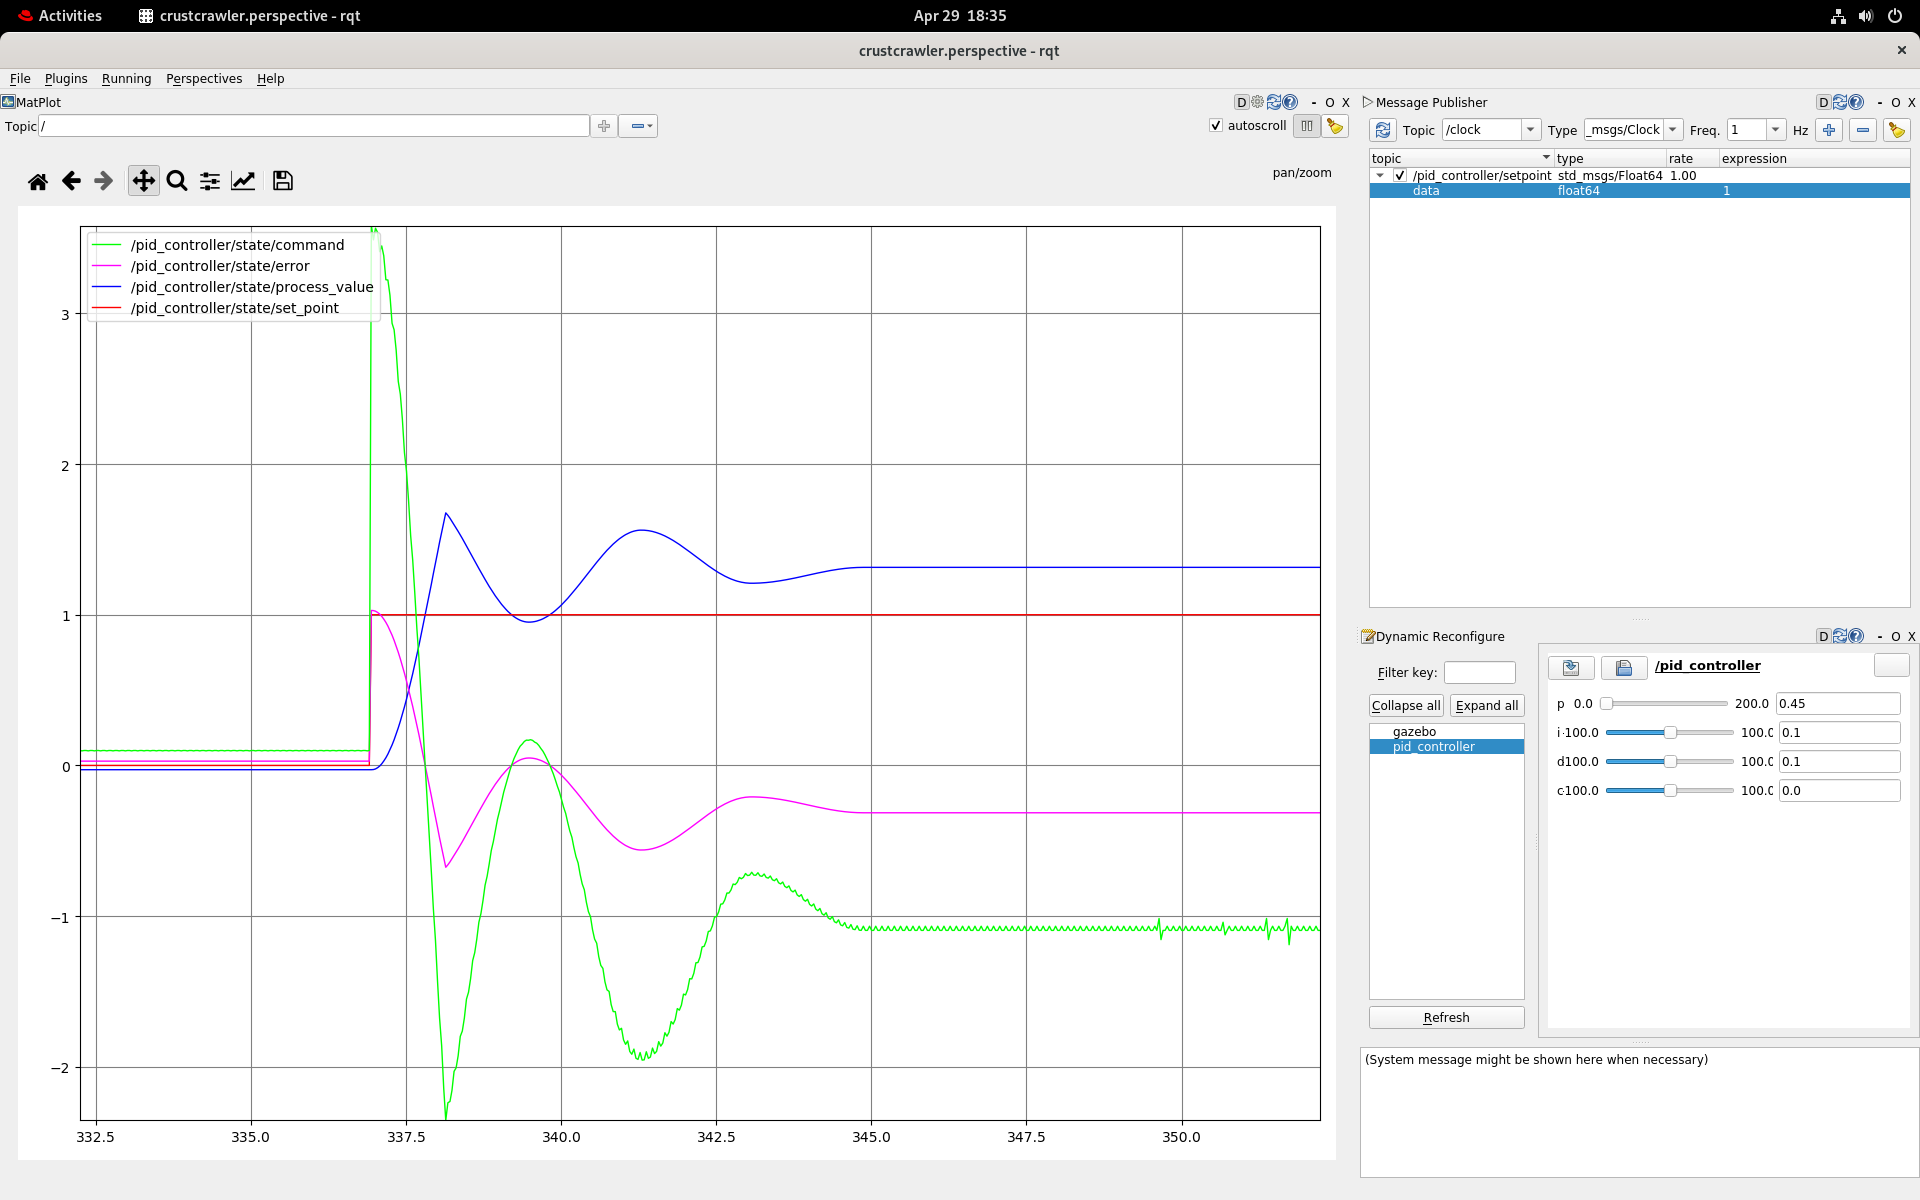
\includegraphics[width=0.8\textwidth]{PI.png}\\
    Frå oppskrift:
    \[T_k = \frac{1}{f_k} = \frac{\pi}{6} = 1.046\]
    \[K_pk = 0.45\]
    Som gir:\\
    \[K_p = 0.27 \hspace{10mm} T_i = 0.523 \hspace{10mm} T_d = 0.00552\]
    Og:\\
    \[K_i = 0.516 \hspace{10mm} K_d = 0.00149\]

    \newpage
    \section{Oppgåve}
    Eg endra i filane oppgitt i oppgåve 3 (i pid\_assignment) for å justere pakkane.
    Endra slik at både 1. og 2. rotasjonsledd kunne bevege seg.
    Da snurra roboten i simulatoren når eg endra 'expression'.
    Ved verdi 1.65 roterte roboten slik at han akuratt nådde nedi bakken rundt seg, 
    og roterte rundt si egia akse. og deermed laga ei sirkel\\
    Filene heiter: \\

    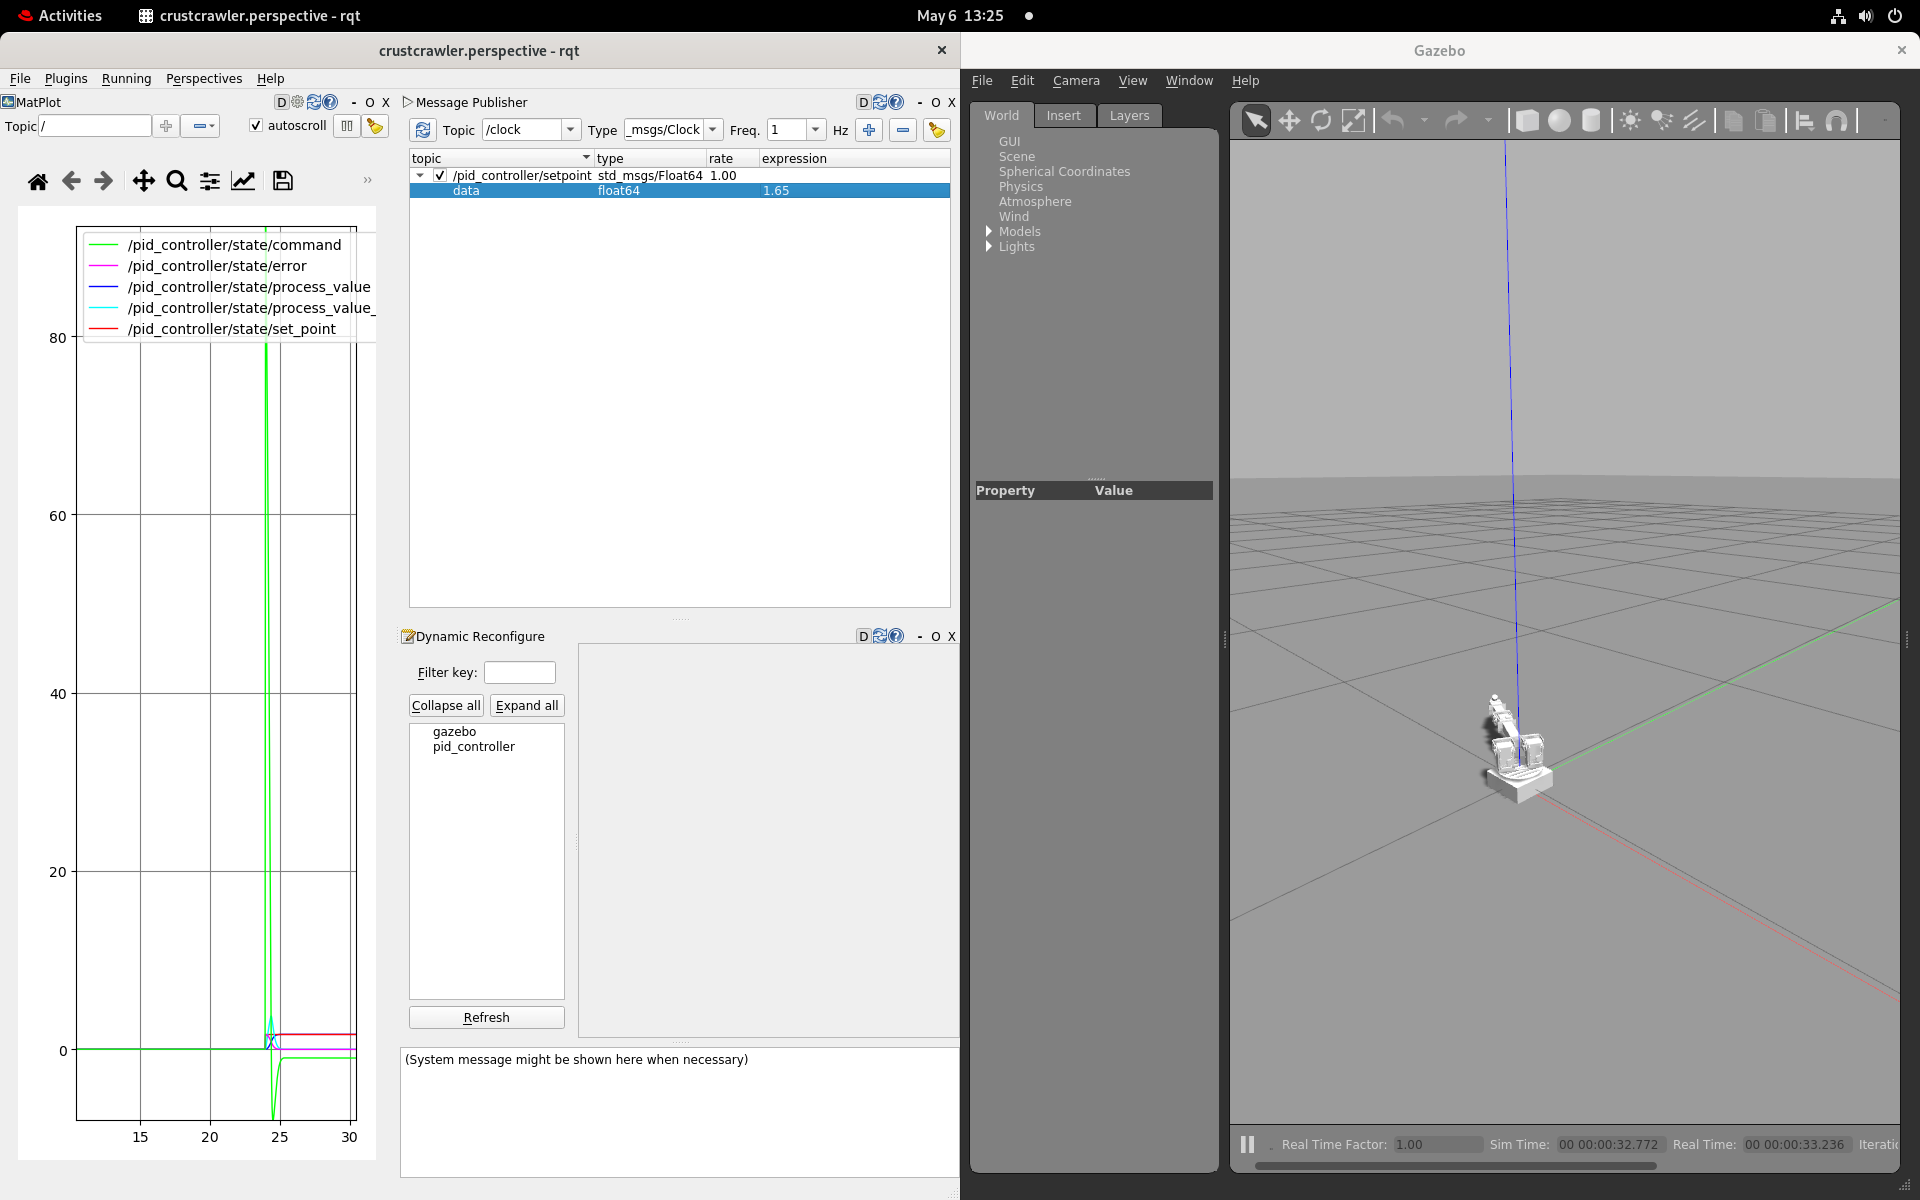
\includegraphics[width=0.8\textwidth]{rot1.png}\\
    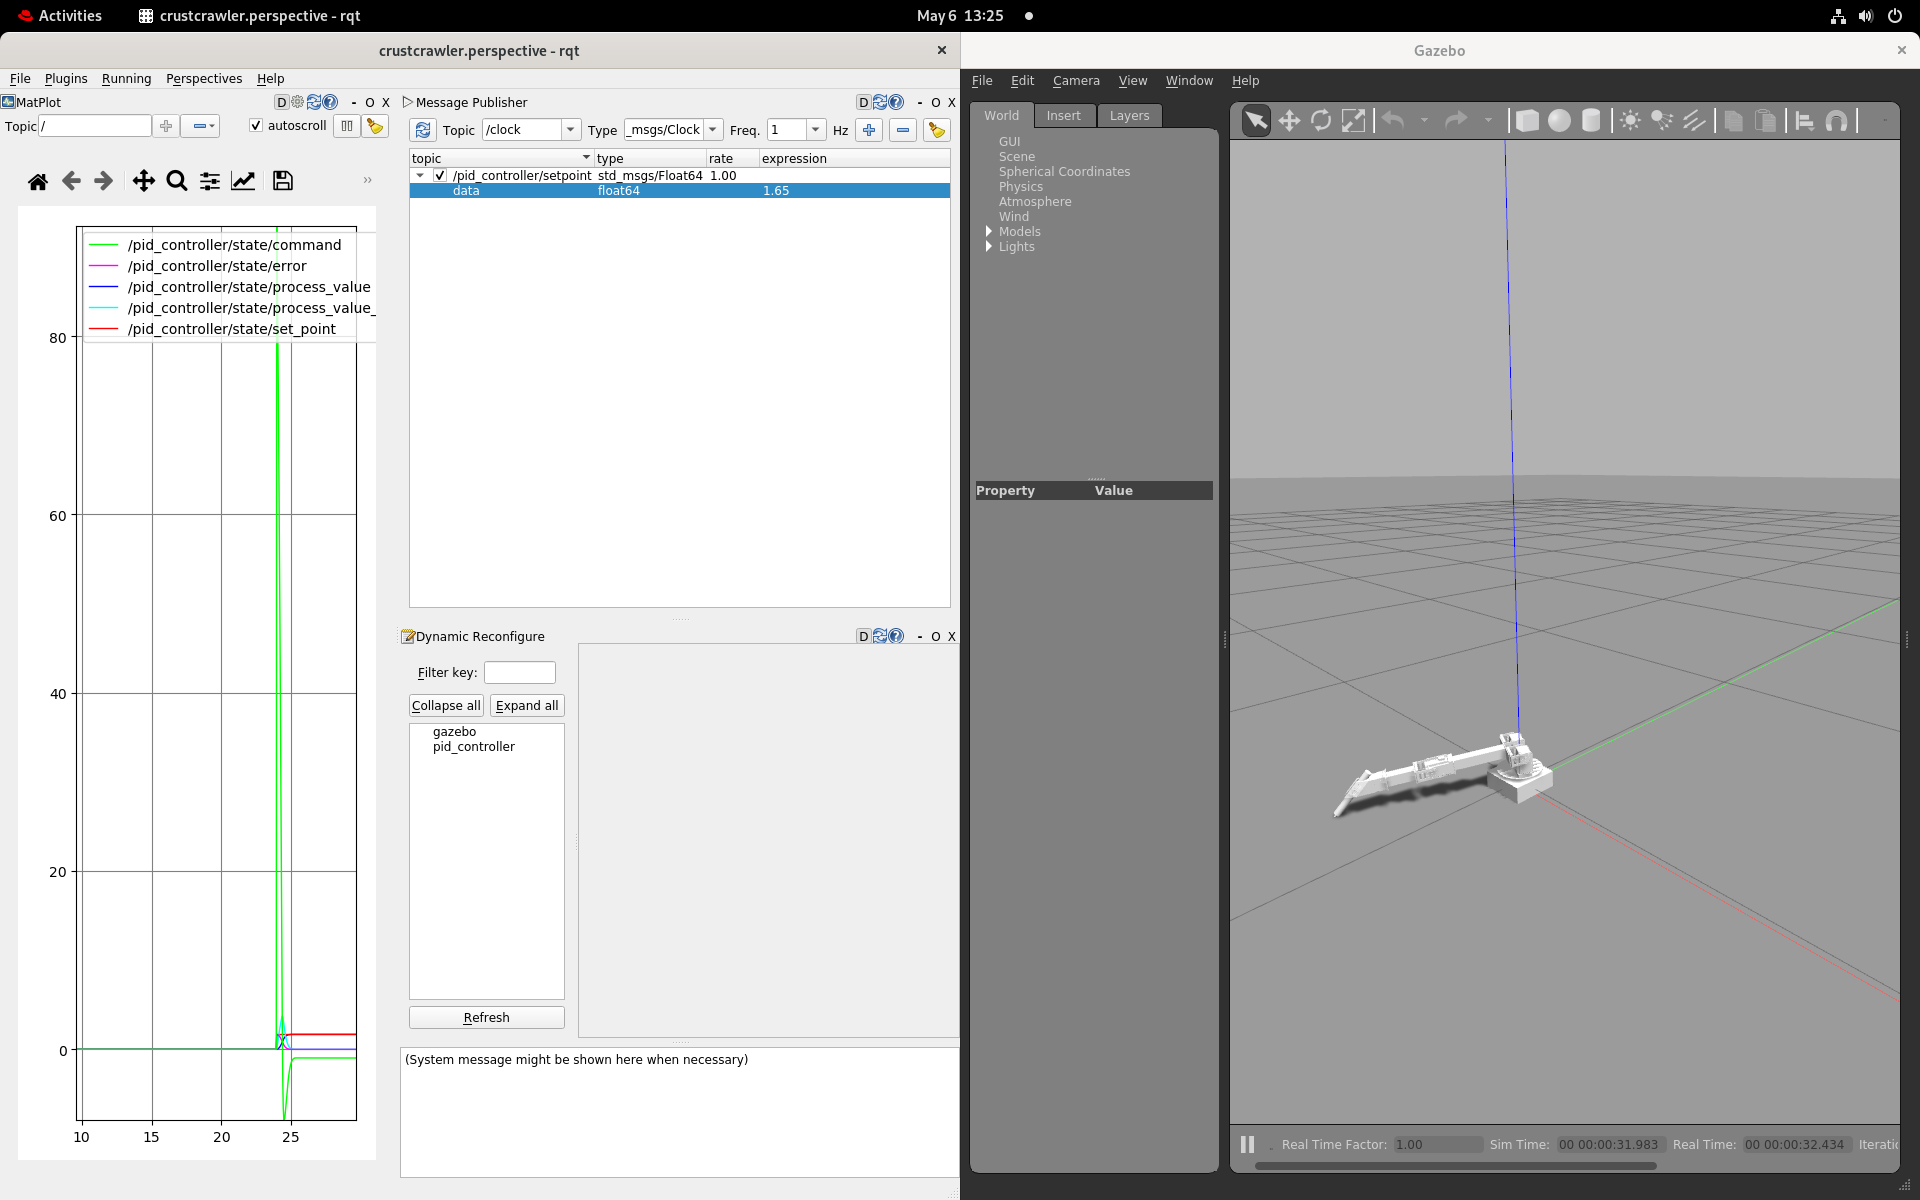
\includegraphics[width=0.8\textwidth]{rot2.png}\\






\end{document}